\iffalse
In diesem Kapitel wird die konkrete Implementierung des im Kapitel
\ref{cha:loesungskonzept} entwickelten Lösungskonzepts beschrieben.
Hierbei wird auf die konkret verwendeten Entwicklungswerkzeuge etc. 
Bezug genommen.

Bei Software-Projekten besteht dieses Kapitel typischerweise aus den 
Phasen Implementierung \& Test im \ac{rup}.

Zum Beispiel kann man hier auch ein kleines Listing einfügen.

\begin{lstlisting}[language=c,%
                   caption={Überschrift des Quelltexts}]
#include<stdio.h>

int main() {
    // Kommentar
    int answer = 20 << 1;
    answer += 2;
    printf("Hallöchen Welt!\n");
    printf("Die Antwort ist: %d\n", answer);
    return 0;
}
\end{lstlisting}

Manchmal hilft auch eine kleine Tabelle:

\begin{table}[htbp]
\centering
\begin{tabular}{|l|r|}
\hline
\textbf{Messwert a} & \textbf{Messwert b} \\ \hline
9 & 5 \\ \hline
1 & 4 \\ \hline
1 & 3 \\ \hline
\end{tabular}
\caption{Überschrift der Tabelle}
\label{tab:my-table}
\end{table}

Details siehe Tabelle~\ref{tab:my-table}.
\fi

Das erarbeitete Lösungskonzept wurde anschließend mit den zuvor beschriebenen Technologien umgesetzt.
Die konkrete Implementierung sieht dabei wie folgt aus:

\section{Backend}
\label{sec:backend}

Im Folgenden werden die einzelnen Dateien und Klassen des Backends beschrieben.
Begonnen wird mit dem Endpunkt in app.py, von welchem aus das DatabaseAnalysis Objekt erstellt wird.
Von diesem ausgehend werden alle weiteren Klassen von außen nach innen beleuchtet.

\subsection{Endpunkte}
\label{sub:ba_endpunkte}

Der bereits beschriebene einzige Endpunkt im Backend ließt in Zeile 6 bis 9 alle benötigten Werte aus dem Request Body aus.
Mit diesen Daten wird dann ein neues Objekt vom Typ DatabaseAnalysis erstellt.
In diesem Objekt wird anschließend die Funktion connect aufgerufen, welche versucht, sich mit der spezifizierten MongoDB Datenbank zu verbinden.
Wenn die Verbindung erfolgreich ist, wird die Datenbank daraufhin analysiert.
Das Resultat der Analyse wird als JSON in der Response zurückgegeben
Im Fehlerfall wird der Response Code 406 zurückgegeben.

\begin{lstlisting}[language=python, caption={app.py},label={lst:backend_app}]
app = Flask("Mongodb Visualization Tool")
CORS(app)

@app.post("/connect")
def get_tables_and_keys():
    connection_string = request.json.get("connection_string")
    database_name = request.json.get("database")
    analyse_ref = request.json.get("analyse_ref")
    sort_method = request.json.get("sort_method")

    db_analysis = DatabaseAnalysis(connection_string, database_name, analyse_ref, sort_method)
    connection_successful = db_analysis.connect()
    if not connection_successful:
        return Response(status=406)

    document_dict = db_analysis.analyse()

    return json.dumps(document_dict)
\end{lstlisting}

\subsection{DatabaseAnalysis}
\label{sub:ba_database_analysis}

Die Methode connect der Klasse DatabaseAnalysis nutzt  den MongoDB Client, um eine Verbindung zu einer MongoDB Datenbank mit dem spezifizierten Connection String und dem Datenbanknamen herzustellen.
Wenn die Verbindung nach 5 Sekunden noch nicht steht, wird der Versuch abgebrochen und False zurückgegeben.
Ansonsten werden die verbundene Datenbank und der verbundene Client im Objekt gespeichert und True zurückgegeben.

\begin{lstlisting}[language=python, caption={DatabaseAnalysis.connect},label={lst:backend_connect}]
def connect(self, connection_string, database):
    try:
        self.mongodb_client = MongoClient(connection_string, serverSelectionTimeoutMS=5000)
        self.database = self.mongodb_client[database]
    except pymongo.errors.ServerSelectionTimeoutError:
        return False
    return True
\end{lstlisting}

In der Methode analyse derselben Klasse werden daraufhin alle Collection Namen in der Datenbank ausgelesen.
Für jeden Namen wird die Collection mit diesem Namen als Dictionary ausgelesen.
Dieses Dictionary enthält wiederum alle Dokumente der Collection.
Jedes Dokument wird in der Methdode ProcessedCollection.add\_doc analysiert und, falls noch nicht vorhanden, der ProcessedCollection hinzugefügt.
Danach werden die ProcessedCollections nachbearbeitet.
Dies beinhaltet Schritte wie beispielsweise das Sortieren der Dokumente und das Markieren der Abweichungen von dem Hauptschema.
Wenn alle Dokumente durchlaufen wurden, wird die Verbindung zur Datenbank geschlossen und die ProcessedCollection wird in ein Dictionary umgewandelt und zurückgegeben.

\begin{lstlisting}[language=python, caption={DatabaseAnalysis.analyse},label={lst:backend_analyse}]
def analyse(self):
    self.collection_names = self.database.list_collection_names()
    docs_dict = {"collections": []}
    for name in self.collection_names:
        processed_collection = ProcessedCollection(name)
        collection = self.database.get_collection(name)
        documents = collection.find({})
        for document in documents:
            processed_collection.add_doc(document)

        processed_collection .post_processing(sort_method=self.sort_method)
        if self.analyse_ref:
            self.analyse_references(processed_collection)
        docs_dict["collections"] .append(processed_collection.to_dict())
    self.mongodb_client.close()
    return docs_dict
\end{lstlisting}

Die Methode analyse\_references in DatabaseAnalysis wird nur ausgeführt, wenn der im Endpunkt übergebene Wert analyse\_ref auf True gesetzt ist.
In der Methode selbst werden alle Values aller verarbeiteten Dokumente durchlaufen und überprüft, ob es sich dabei um eine Referenz auf ein anderes Dokument handeln könnte.
Wenn der Datentyp des Values Object ID ist und der Name des Values nicht \_id entspricht (Es sich also nicht um den Primary Key handelt), wird angenommen, dass der Value eine Referenz ist.
Wenn dies der Fall ist, werden aus den Originaldokumenten, die im verarbeiteten Dokument abgespeichert sind, die Werte der soeben identifizierten Referenz ausgelesen.
Mit diesen Werten wird dann get\_referenced\_collection so lange aufgerufen, bis die Methode einmal nicht None zurückgibt.
get\_referenced\_collection durchläuft die \_id Werte aller (unverarbeiteten) Dokumente und vergleicht diese mit der übergebenen Object ID.
Sobald eine Übereinstimmung gefunden wird, wird der Name der Collection zurückgegeben, in der sich das Dokument mit der passenden \_id befindet.
Wenn keine Übereinstimmung gefunden wird, dann wird None zurückgegeben.

\begin{lstlisting}[language=python, caption={DatabaseAnalysis.analyse\_references},label={lst:backend_analyse_ref}]
def analyse_references(self, processed_collection):
    for document in processed_collection.documents:
        for value in document.values:
            if value.val_type == "Object ID" and value.key != "_id":
                for orig_document in document.original_documents:
                    referenced_collection = self.get_referenced_collection (orig_document.get(value.key))
                    if referenced_collection is not None:
                        value.ref = referenced_collection
                        return

def get_referenced_collection(self, _id):
    for collection_name in self.collection_names:
        collection = self.database.get_collection(collection_name)
        document = collection.find_one({"_id": _id})
        if document is not None:
            return collection_name
    return None
\end{lstlisting}

Die Bestimmung der Referenzen mit dieser Methode ist nicht immer akkurat, da der Primary Key eines Schemas auch einen anderen Datentyp als Object ID haben kann.
Da die Bestimmung der Referenzen sonst jedoch sehr komplex und rechenintensiv werden würde, werden die Referenzen in dieser Arbeit nur mit dieser vereinfachten Methode analysiert.

\subsection{ProcessedCollection}
\label{sub:ba_processed_collection}

Die Methode add\_doc in der Klasse ProcessedCollection erstellt aus dem übergebenen Dokument in Form eines Dictionary ein neues Objekt der Klasse ProcessedDocument.
Wenn sich noch kein Objekt mit den gleichen Werten in der aktuellen ProcessedCollection befindet, wird das ProcessedDocument der ProcessedCollection hinzugefügt.
Ansonsten wird das Attribut count in dem bereits vorhandenen ProcessedDocument Objekt hochgezählt.


\begin{lstlisting}[language=python, caption={ProcessedCollection.add\_doc},label={lst:backend_add_doc}]
def add_doc(self, document):
    new_doc = ProcessedDocument(document)
    for doc in self.documents:
        if doc == new_doc:
            doc.count += 1
            if doc.document_ages:
                doc.document_ages .append(new_doc.document_ages[0])
            doc.original_documents .append(new_doc.original_documents[0])
            return
    self.documents.append(new_doc)
\end{lstlisting}

Darüber hinaus enthält ProcessedCollection die methode post\_processing.
Post\_processing ruft Methoden auf, welche die ProcessedDocuments in dieser ProcessedCollection nachbearbeiten.
Folgende Nachbearbeitungsschritte werden ausgeführt:
\begin{enumerate}
    \item Durchschnittliches Alter aller Dokumente eines ProcessedDocuments ausrechnen
    \item Dokumente nach dem Durchschnittsalter oder nach der Anzahl der Aufrufe sortieren
    \item Zusätzliche Werte gegenüber dem Hauptschema ermitteln (das Hauptschema ist das Schema, welches in der Sortierung an oberster Stelle steht)
    \item Fehlende Werte gegenüber dem Hauptschema ermitteln
\end{enumerate}

\begin{lstlisting}[language=python, caption={ProcessedCollection.post\_processing},label={lst:backend_post_processing}]
def post_processing(self, sort_method):
    self.calc_document_averages()
    self.sort_documents(sort_method)
    self.mark_additional_values()
    self.mark_missing_values()

def calc_document_averages(self):
    for document in self.documents:
        if document.document_ages:
            document.avg_age = sum(document.document_ages) / len(document.document_ages)

def sort_documents(self, sort_method):
    if sort_method == "documentCount":
        self.documents = sorted(self.documents, key=lambda document: document.count, reverse=True)
    elif sort_method == "avgAge":
        self.documents = sorted(self.documents, key=lambda document: document.avg_age, reverse=True)

def mark_additional_values(self):
    main_doc = self.documents[0]
    for i in range(1, len(self.documents)):
        for value in self.documents[i].values:
            if value not in main_doc.values:
                value.is_additional = True

def mark_missing_values(self):
    main_doc = self.documents[0]
    for i in range(1, len(self.documents)):
        for value in main_doc.values:
            if value not in self.documents[i].values:
                self.documents[i] .missing_values.append(value.key)
\end{lstlisting}

\subsection{ProcessedDocument}
\label{sub:ba_processed_document}

Sämtliche Logik in der ProcessedDocument Klasse steckt im Konstruktor.
Der Konstruktor nimmt ein Dokument im JSON Format entgegen.
In diesem Dokument werden mithilfe der Methode analyse\_values in der Datei value.py alle Werte analysiert und die Ergebnisse als Liste des eigenen Datentyps Value im ProcessedDocument gespeichert.
Wenn der Primary Key vom Typ Object ID ist, wird in Zeile 6 bis 8 das Alter des Dokuments ermittelt und in einer Liste gespeichert.
Diese Liste dient später dazu, das Durchschnittsalter des ProcessedDocuments zu berechnen.
Das Bestimmen des Alters eines Dokuments ist nur möglich, wenn der Primary Key vom Typ Object ID ist, da Object IDs einen Zeitstempel beinhalten.
Des Weiteren initialisiert der Konstruktor noch einige Werte, die für die Nachbearbeitung benötigt werden.

\begin{lstlisting}[language=python, caption={ProcessedDocument.\_\_init\_\_},label={lst:backend_processed_document_init}]
def __init__(self, document):
    self.values = analyse_values(document)
    self.count = 1
    self.document_ages = list()
    _id = document.get("_id")
    if isinstance(_id, bson.ObjectId):
        document_generation_time = document.get("_id").generation_time
        document_age = (datetime.datetime.now(datetime.timezone.utc) - document_generation_time).total_seconds()
        self.document_ages.append(document_age)
    self.avg_age = None
    self.missing_values = list()
    self.original_documents = list()
    self.original_documents.append(document)
\end{lstlisting}

\subsection{Value}
\label{sub:ba_value}

Die Methode analyse\_values in value.py ist eine Factory Methode, welche für alle Key Value Paare im übergebenen Dokument-Dictionary einen Value erstellt und als Liste zurückgibt.

\begin{lstlisting}[language=python, caption={Value.analyse\_values},label={lst:backend_value_analyse_values}]
def analyse_values(document):
    values = list()
    for key, value in zip(document, document.values()):
        value = Value(key, value)
        values.append(value)
    return values
\end{lstlisting}

Der Konstruktor der Value Klasse initialisiert alle im ER-Diagramm beschriebenen Values und analysiert den Datentyp des Values mit der Methode get\_type.
Darüber hinaus wird im Konstruktor überprüft, ob es sich bei dem Value um ein verschachteltes Dokument oder ein Array handelt. 
Wenn dies der Fall ist, werden die entsprechenden Analysemethoden aufgerufen.

\begin{lstlisting}[language=python, caption={Value.\_\_init\_\_},label={lst:backend_value_init}]
def __init__(self, key, raw_value):
    self.key = key
    self.ref = None
    self.nested_document = None
    self.array_values = None
    self.val_type = get_type(raw_value)
    self.is_additional = False
    if self.val_type == "Embedded document":
        self.nested_document = analyse_values(raw_value)
    elif self.val_type == "Array":
        self.analyse_array(raw_value)
\end{lstlisting}

get\_type enthält simple If-Bedingungen, welche den Python-Datentyp eines Werts zu einem String mappen.
Dieser String entspricht dem MongoDB-Datentyp des Werts.
Wenn der Datentyp nicht von den If-Bedingungen abgedeckt wird, wird eine Exception geworfen.

\begin{lstlisting}[language=python, caption={Value.get\_type},label={lst:backend_value_get_type}]
def get_type(value):
    if value is None or type(value) is None:
        return "Null"
    if isinstance(value, str):
        return "String"
    if isinstance(value, bson.ObjectId):
        return "Object ID"
    if isinstance(value, bool):
        return "Boolean"
    if isinstance(value, (int, float, complex, bson.Decimal128)):
        return "Number"
    if isinstance(value, datetime.date):
        return "Date"
    if isinstance(value, collections.abc.Sequence):
        return "Array"
    if isinstance(value, dict):
        return "Embedded document"
    raise Exception(f"Type {type(value)} of value {value} is not identifiable!")
\end{lstlisting}

Wenn es sich bei dem Datentyp des Values um ein Array handelt, wird für jeden Wert im Array ein Value-Objekt erstellt.
Die Besonderheit bei Value-Objekten in einem Array ist, dass das Feld Key leer bleibt, da Values in Arrays keinen eigenen Key besitzen.
Wenn das Array array\_values des darüberliegenden Values noch keinen Value enthält, der den gleichen Datentyp hat, wird das eben erzeugte Value-Objekt in array\_values gespeichert.

\begin{lstlisting}[language=python, caption={Value.analyse\_array},label={lst:backend_value_analyse_array}]
def analyse_array(self, raw_value):
    self.array_values = list()
    for arr_element in raw_value:
        array_value = Value(None, arr_element)
        self.add_array_value(array_value)

def add_array_value(self, new_array_value):
    for array_value in self.array_values:
        if array_value == new_array_value:
            return
    self.array_values.append(new_array_value)
\end{lstlisting}

\section{Frontend}
\label{sec:frontend}

\subsection{Startbildschirm und Auswahl des Tools}
\label{sub:fe_startbildschirm}

Die Gesamtlösung des Frontends besteht aus mehreren Tools, die zu einer Toolbox für Datenbanken zusammengefasst werden.
Um auswählen zu können, welches Tool man benutzen will, wurde ein Startbildschirm eingefügt.
Der Startbildschirm ist ein simples HTML div, welches den Titel der Anwendung sowie Buttons beinhaltet.
Die Buttons sind mit den Namen der einzelnen Tools beschriftet.
Die onClick Funktionen der Buttons rufen die Funktion switchAppMode auf, welche als Parameter das enum AppScreen übergeben bekommt.
AppScreen teilt der Funktion wiederum mit, welches Tool ausgewählt wurde und geladen werden muss.
switchAppMode nutzt dann React Router, um zu der entsprechenden URL des Screens zu navigieren.

\begin{figure}[H]
    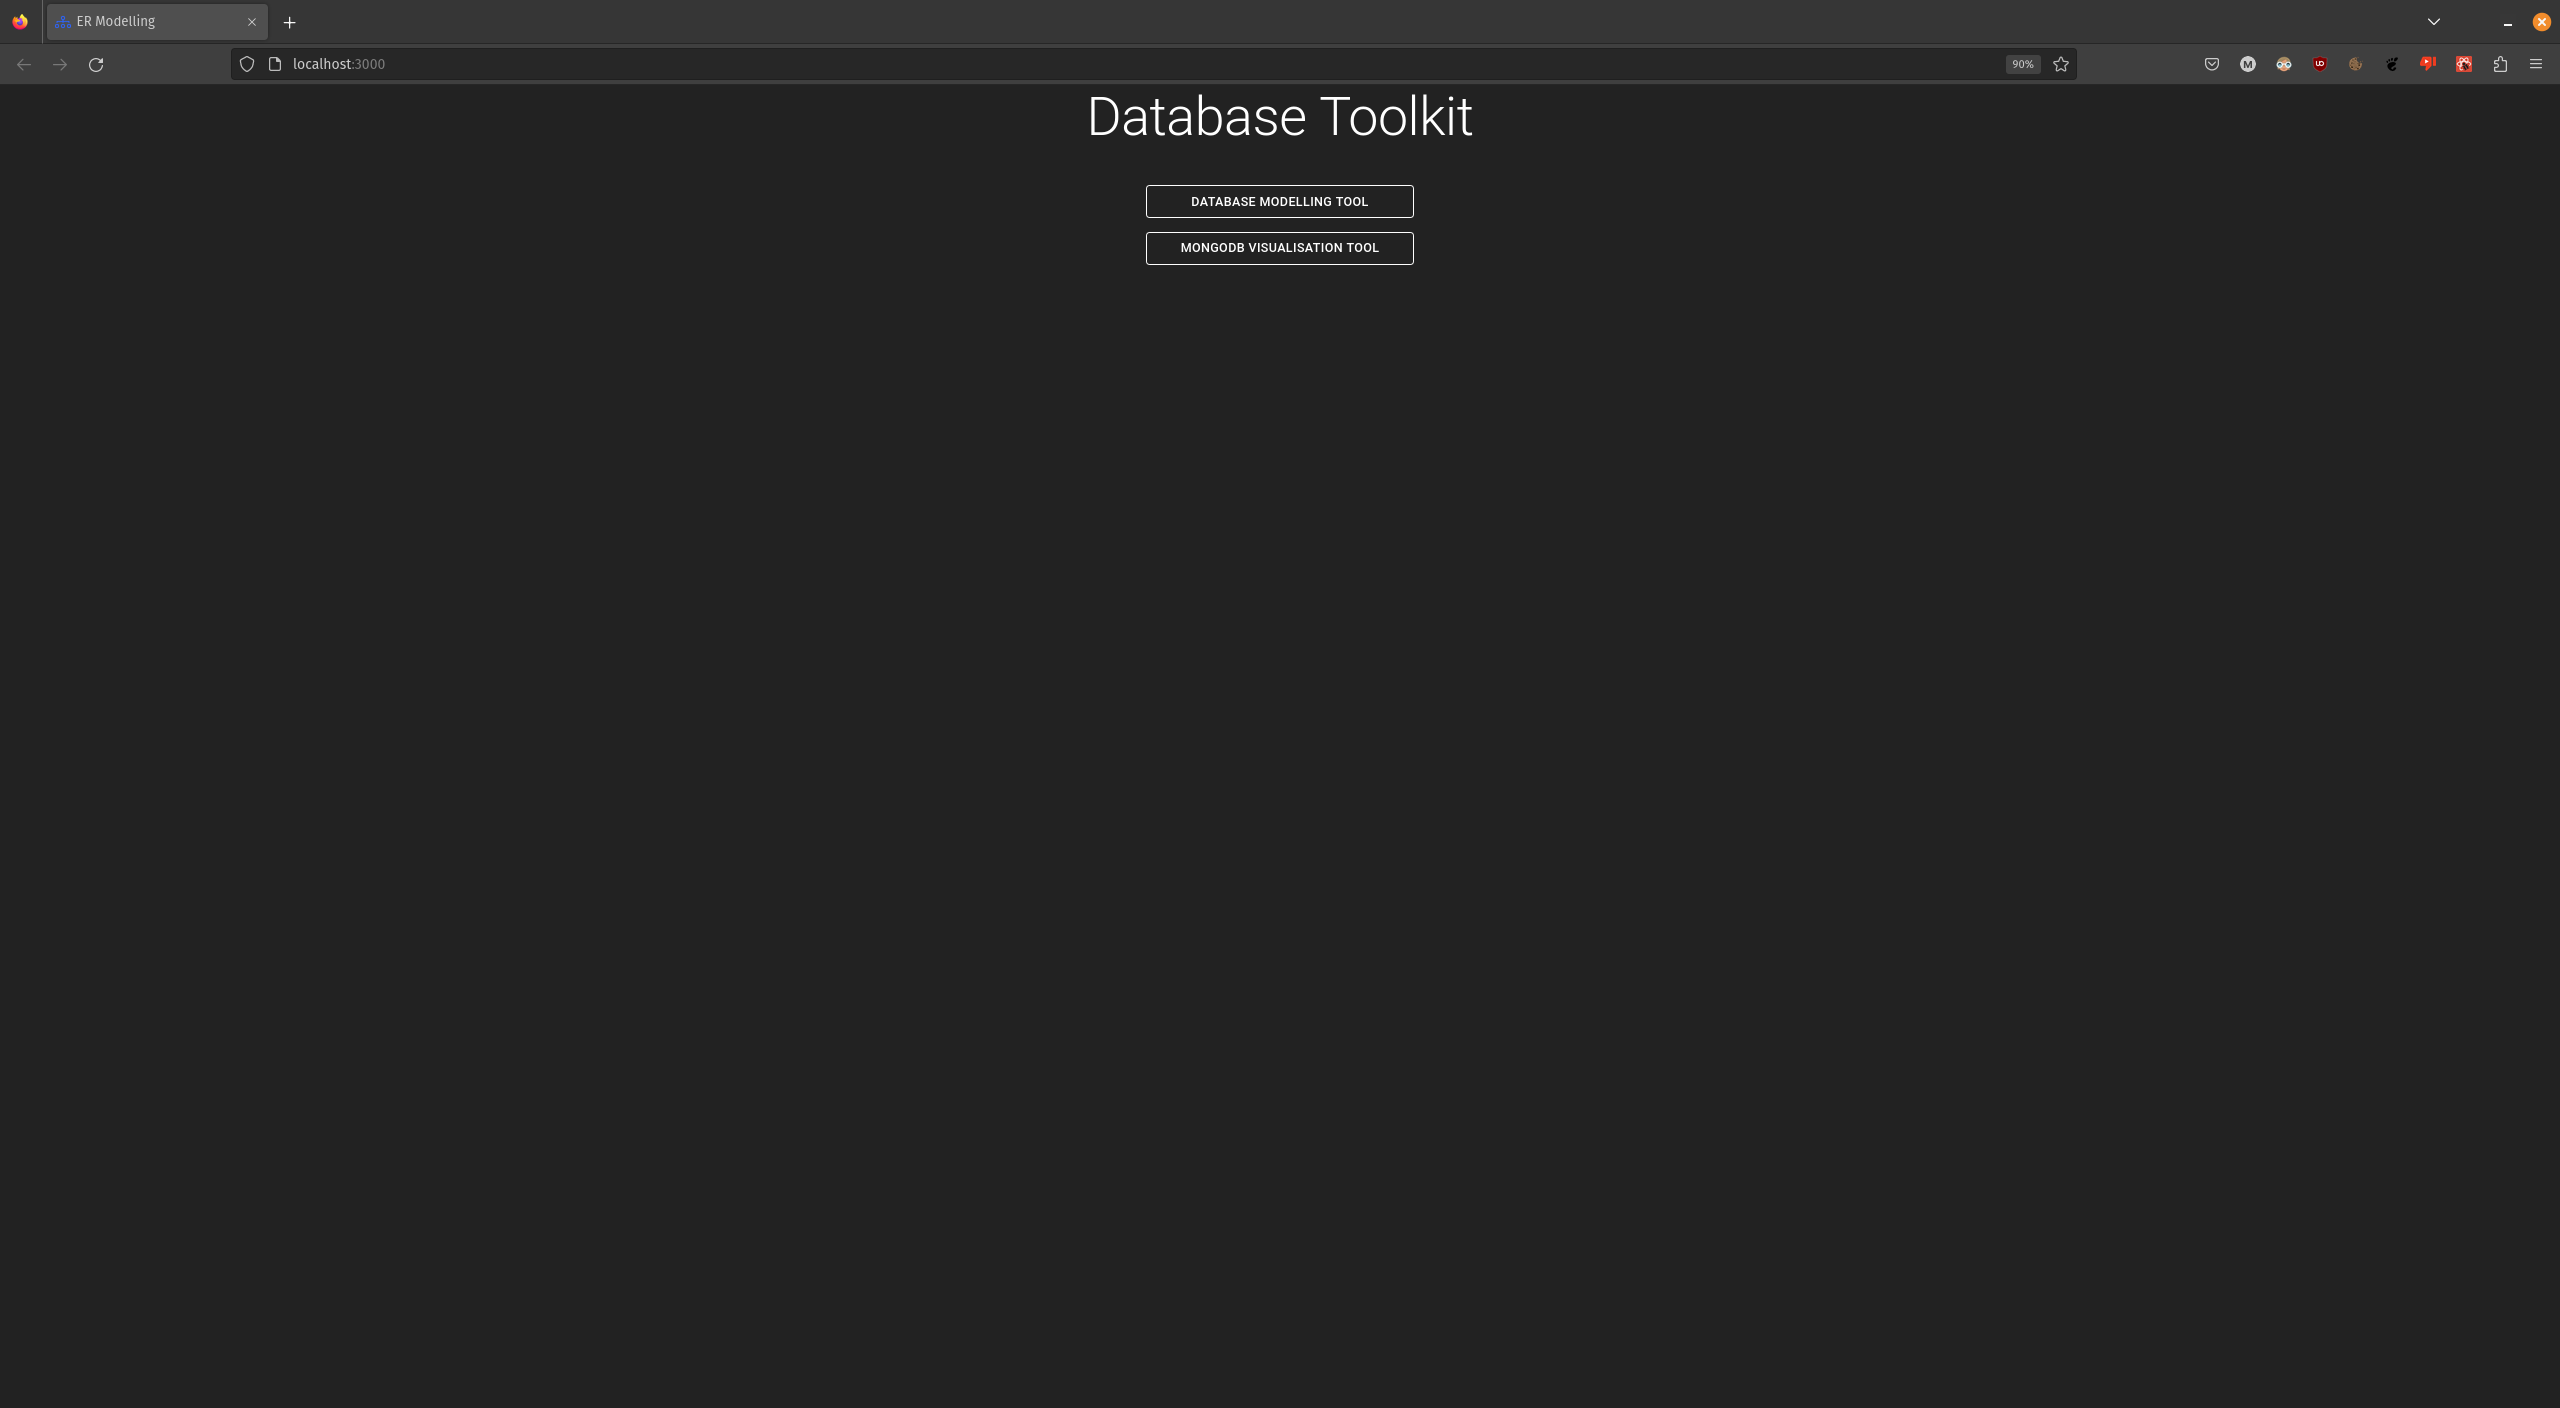
\includegraphics[width=\textwidth]{images/frontend_titlescreen}
    \caption{Frontend Startbildschrim}
    \label{fig:frontend_titlescreen}
\end{figure}

Das Rendern der einzelnen Tool Screens erfolgt daraufhin in der Datei App.js.
Hier wird mittels React Router der Startbildschirm als Index Element definiert, welches initial angezeigt wird.
Zudem wird der Pfad aller weiteren Screens definiert, über welchen diese dann geladen werden können.

\begin{lstlisting}[language=JavaScript, caption={React Router in App.js},label={lst:app.js}]
<BrowserRouter>
    <Routes>
        <Route index element={<TitleScreen/>}/>
        <Route path={AppScreens.dbModellingTool} element={<DatabaseModellingTool/>}/>
        <Route path={AppScreens.mongoVisTool} element={<MongoManager/>}/>
    </Routes>
</BrowserRouter>
\end{lstlisting}

\subsection{Aufbau des MongoDB Visualisation Tool Frontends}
\label{sub:fe_aufbau}
Das oberste Element des MongoDB Visualization Tools ist der MongoManager, welcher die MongoLeftSidebar und das MongoDiagram enthält.
Mithilfe der MongoLeftSideBar kann die Verbindung und Analyse der MongoDB Datenbank konfiguriert und durchgeführt werden.
Nach dem Verbinden und Analysieren werden in dem MongoDiagram DocumentTables angezeigt, welche rekursiv geschachtelt wieder DocumentTables enthalten können.
Darüber hinaus gibt es noch ein DetailView Popup, welches angezeigt wird, wenn man auf den Titel eines DocumentTables klickt.
Die DetailView enthält ebenfalls DocumentTables, welche auch wieder rekursiv geschachtelt sein können.
(Das DetailView Popup ist in der nachfolgenden Grafik nicht abgebildet)

\begin{figure}[H]
    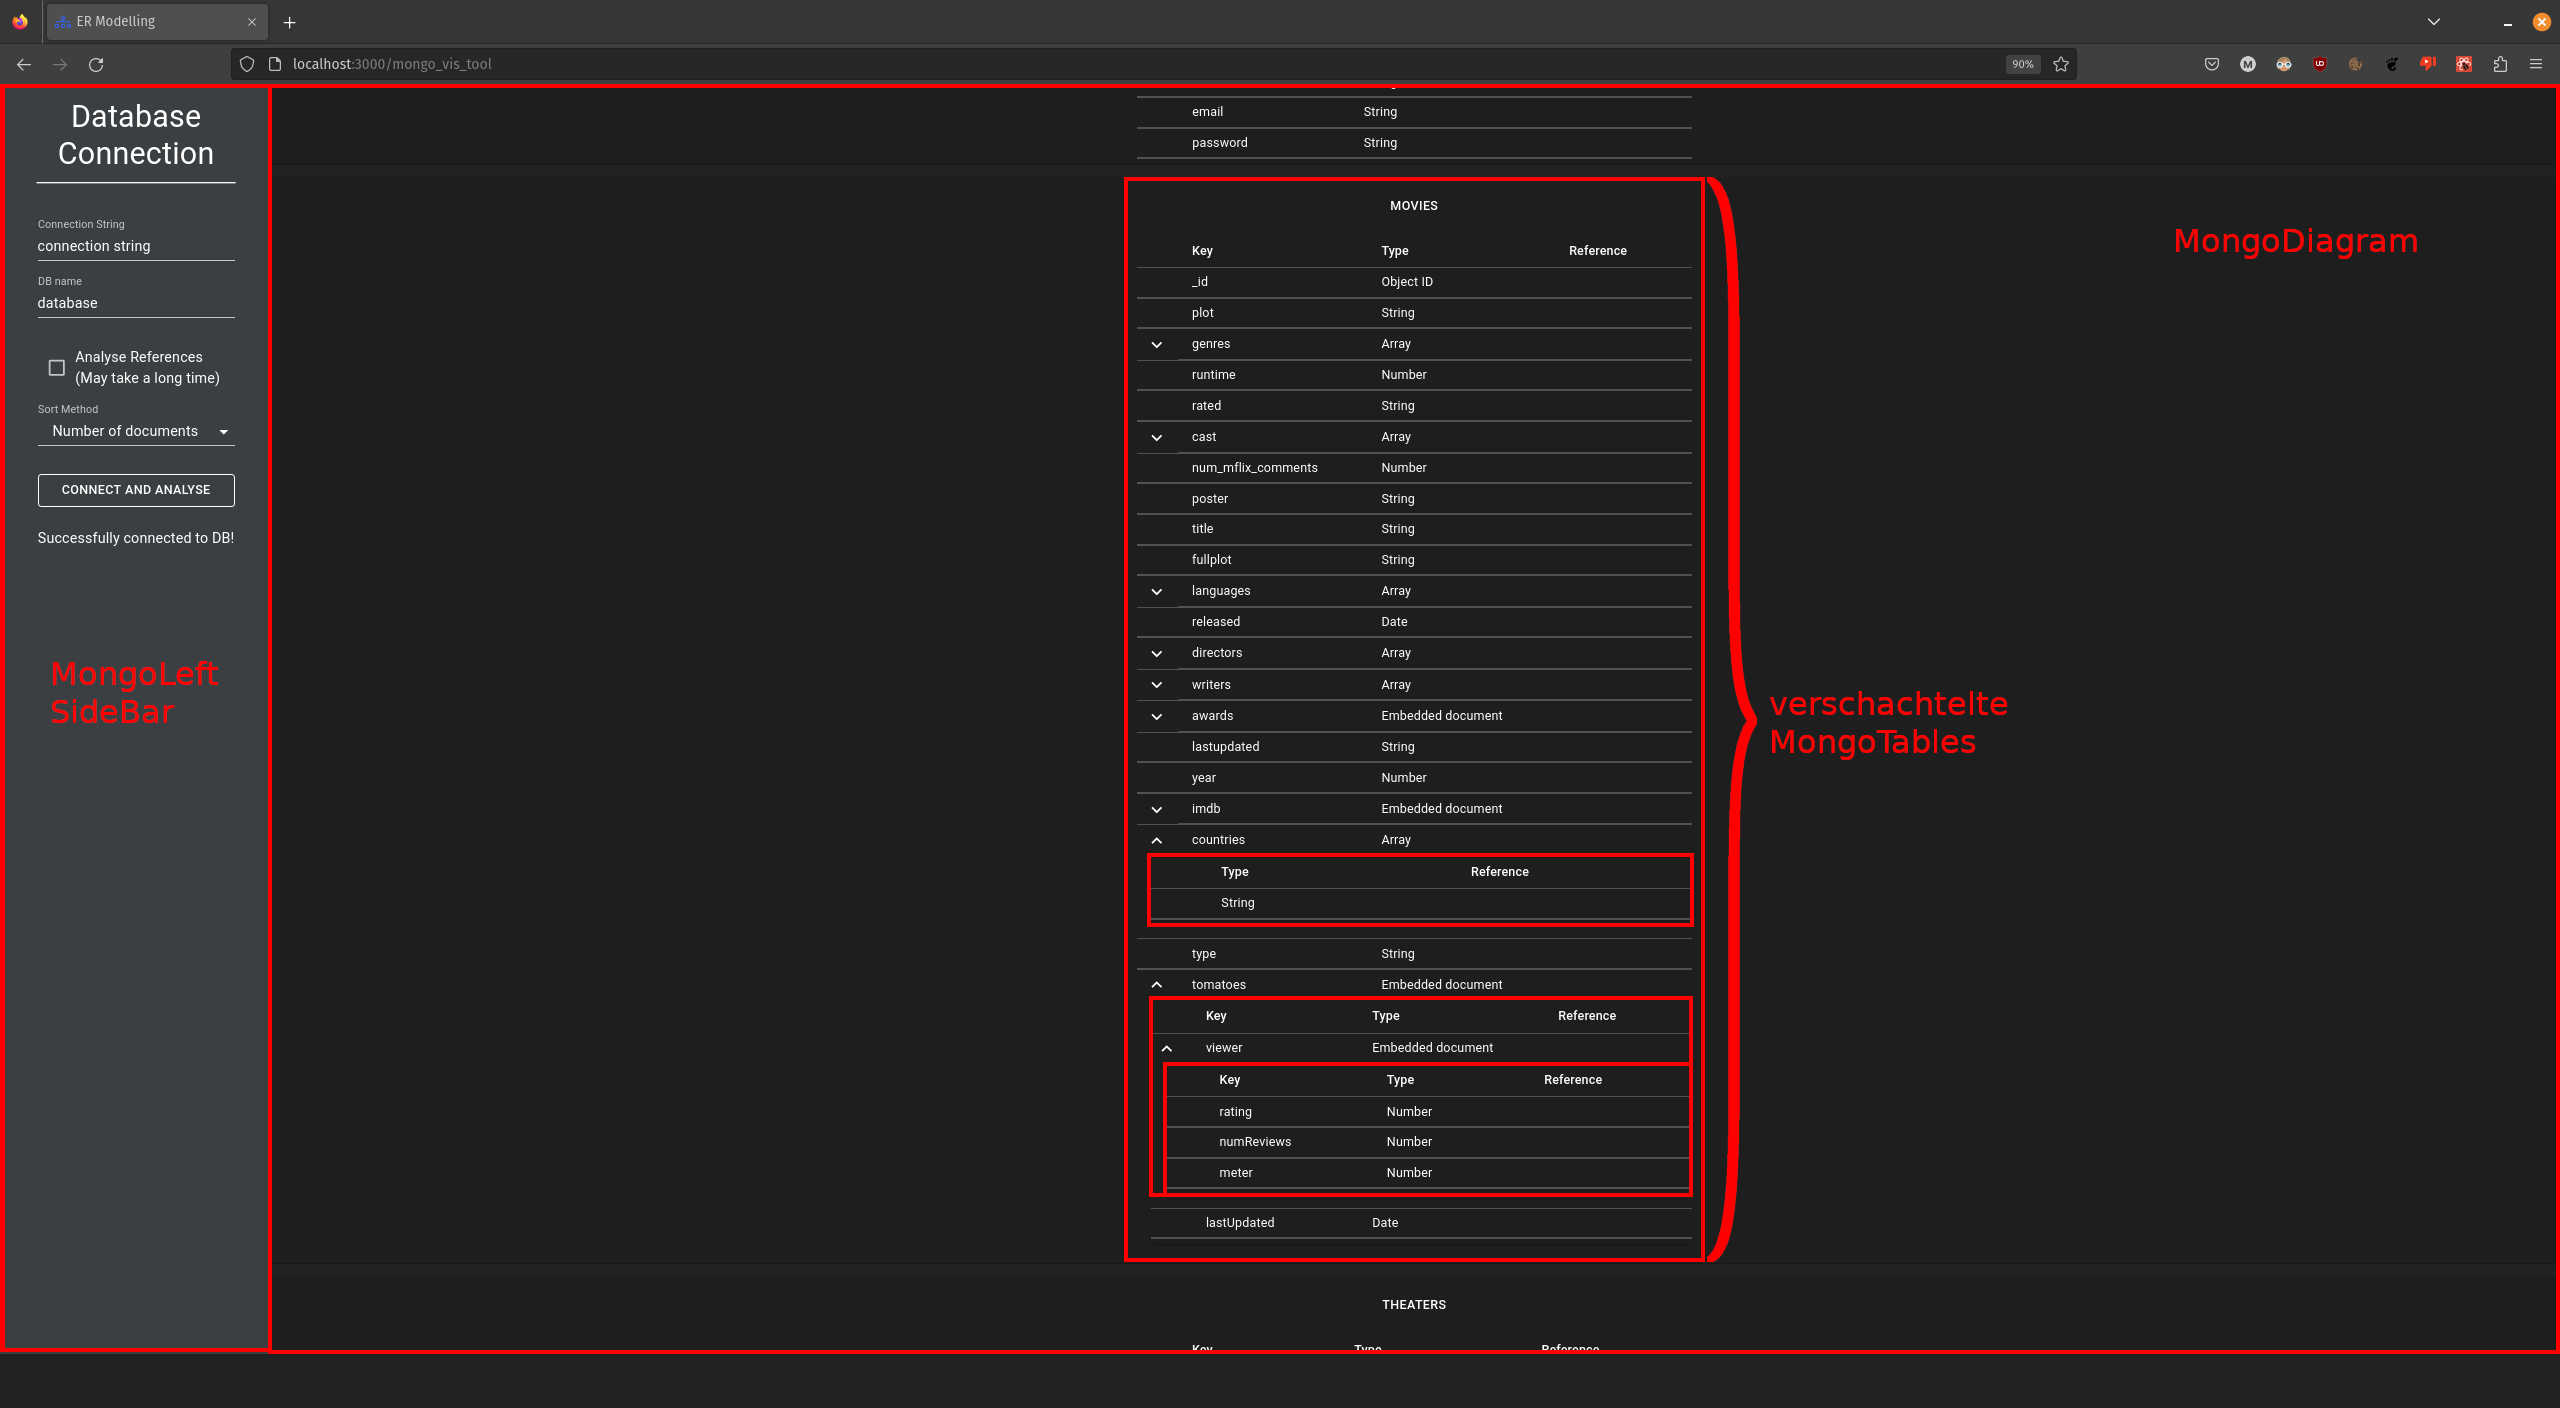
\includegraphics[width=\textwidth]{images/frontend_layers}
    \caption{Frontend Elemente}
    \label{fig:frontend_layers}
\end{figure}

\subsection{Left Sidebar}
\label{sub:fe_left_sidebar}

Die  MongoLeftSideBar nutzt die Material UI Komponenten Typography, TextField, FormControl und Button, um das Eingeben der Verbindungs- und Analysedetails zu ermöglichen.
Diese Informationen werden bei jeder Änderung im State der MongoLeftSideBar gespeichert.
Nach dem Drücken des Connect-Buttons wird die Methode connectToDB aufgerufen.
In dieser Methode wird mit den im State gespeicherten Informationen mithilfe von Axios ein HTTP Request an das Backend gesendet.
Wenn die Verbindung erfolgreich ist, wird die Methode connectionSuccessful aufgerufen.
In dieser werden die analysierten Daten des Backends im ReduxStore gespeichert.
Dies löst im Anschluss das Rendering der DocumentTables im MongoDiagram aus.
Zudem wird das Feedback Label in der MongoLeftSideBar aktualisiert.
Im Fehlerfall wird nur das Feedback Label in der Methode connectionFailed aktualisiert.


%TODO url als Umgebungsvariable abfragen
\begin{lstlisting}[language=JavaScript, caption={MongoLeftSideBar.connectToDB},label={lst:mongo_left_side_bar_connect_to_db}]
function connectToDB() {
    console.log("connecting to db")
    setConnectionState(ConnectionStates.connecting)
    const url = "http://127.0.0.1:5000/connect"

    let contentToSend = {
        connection_string: connectionString,
        database: dbName,
        analyse_ref: analyseRef,
        sort_method: sortMethod
    };

    axios.post(url, contentToSend).then((response) => {
        connectionSuccessful(response)
    }).catch(error => connectionFailed(error))
}

function connectionSuccessful(response) {
    console.log("data: " + response.data)
    setConnectionState(ConnectionStates.connected)
    dispatch(setCollections(response.data))
}

function connectionFailed(error) {
    console.log(error)
    setConnectionState(ConnectionStates.connectionFailed)
}
\end{lstlisting}

\subsection{DocumentTable}
\label{sub:fe_document_table}

Ein DocumentTable repräsentiert ein Schema von Dokumenten in einer Collection.
Es gibt mehrere Arten von DocumentTables, welche je nach Verwendungszweck mit dem Enum DocumentTableType unterschieden werden:
\begin{itemize}
    \item \textbf{main} ist die standard Tabelle, welche im MongoDiagram benutzt wird, um das Hauptschema einer Collection darzustellen.
    \item \textbf{nested} ist eine verschachtelte Untertabelle, entspricht also dem Datentyp Embedded Document.
    \item \textbf{array} wird für den Datentyp Array benutzt.
    \item \textbf{detail} wird im DetailView Popup benutzt, um alle Variatonen der Schemas einer Collection darzustellen.
\end{itemize}

Dem Element DocumentTable liegt die Material UI Table zugrunde.
Material UI Tables haben eine Toolbar, welche hierfür je nach DocumentTableType angepasst wird.
In der Main DocumentTable besteht die Toolbar aus einem Button, mit dem Namen der dargestellten Collection als Label.
Die onClick Methode dieses Buttons öffnet die DetailView dieser Collection.
Wenn der DocumentTableType detail entspricht, zeigt die Toolbar die Anzahl der Dokumente, die dieses Schema benutzen, sowie eventuell die fehlenden Felder gegenüber dem Hauptschema.
In allen anderen Fällen bleibt die Toolbar leer.

Die Spaltenüberschriften im Tablehead sind <Leer> - Key - Type - Reference.
Wenn es sich um ein Array handelt, wird die Spalte Key weggelassen.
Die Reihen selbst haben in der ersten Spalte entweder einen Expand Button, mit dem sich Untertabellen und Arrays ausklappen lassen, oder nichts.
In den nachfolgenden Spalten werden die Daten aus dem Backend eingefüllt.
Nach jeder Reihe folgt eine zunächst unsichtbare Reihe.
Wenn der Datentyp des Werts in dieser Reihe Array oder Embedded document entspricht, wird in dieser unsichtbaren Reihe die entsprechende Untertabelle geladen.
Diese lässt sich dann mit dem Expand Button ausklappen und anzeigen.

\begin{figure}[H]
    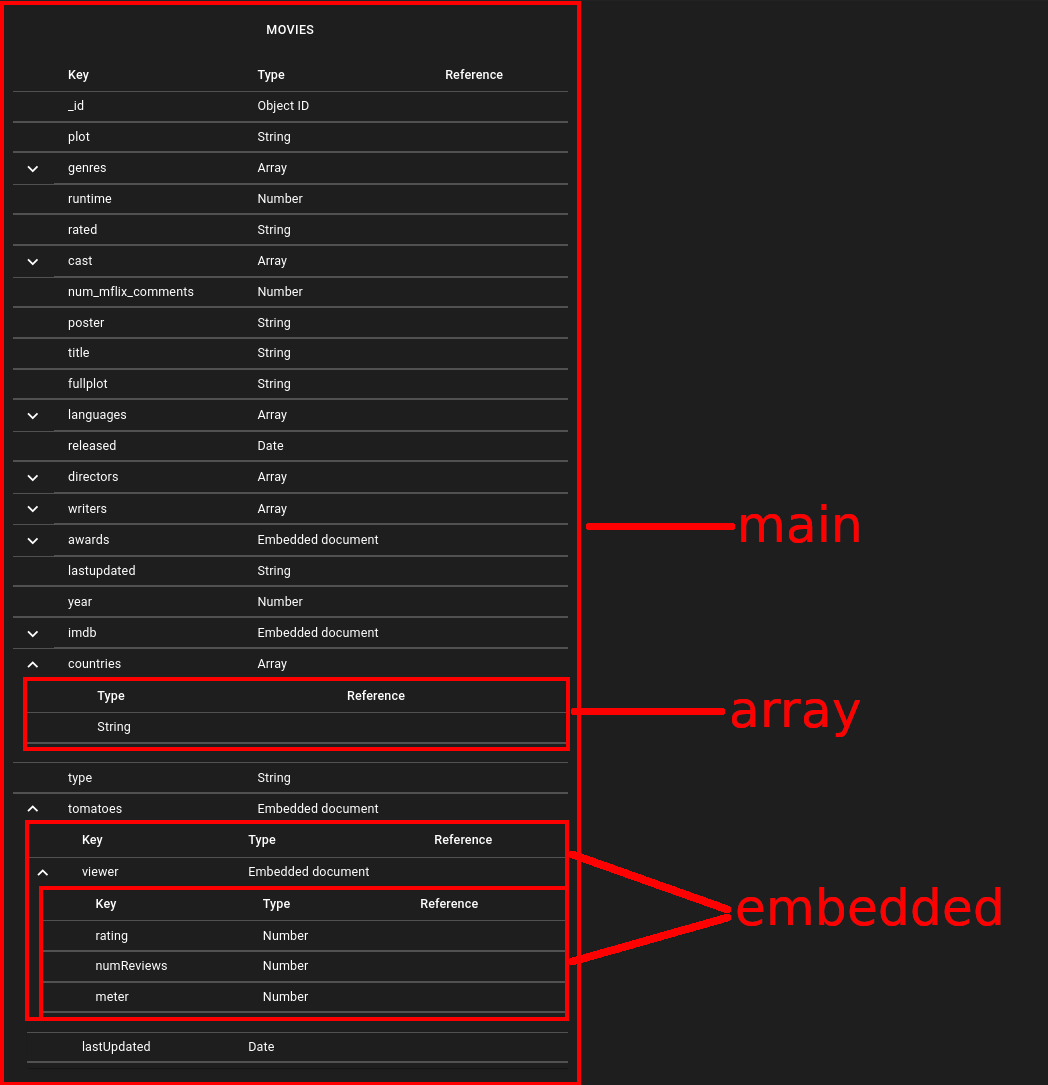
\includegraphics[width=360pt]{images/table_types}
    \caption{Frontend DocumentTable Typen}
    \label{fig:table_types}
\end{figure}

\subsection{DetailView Popup}
\label{sub:fe_detail_view}

Tatsächlich rendert die return Methode des DetailViewPopups zunächst nur einen Button. 
Erst wenn dieser Button gedrückt wird, wird das Popup als Material UI Modal angezeigt.
Dieses Modal lädt daraufhin, wie auch der MongoManager, DocumentTables.
Der DocumentTableType ist in diesen Tabellen jedoch nicht main, sondern detail, was die Toolbars der Tabellen verändert.


\begin{figure}[H]
    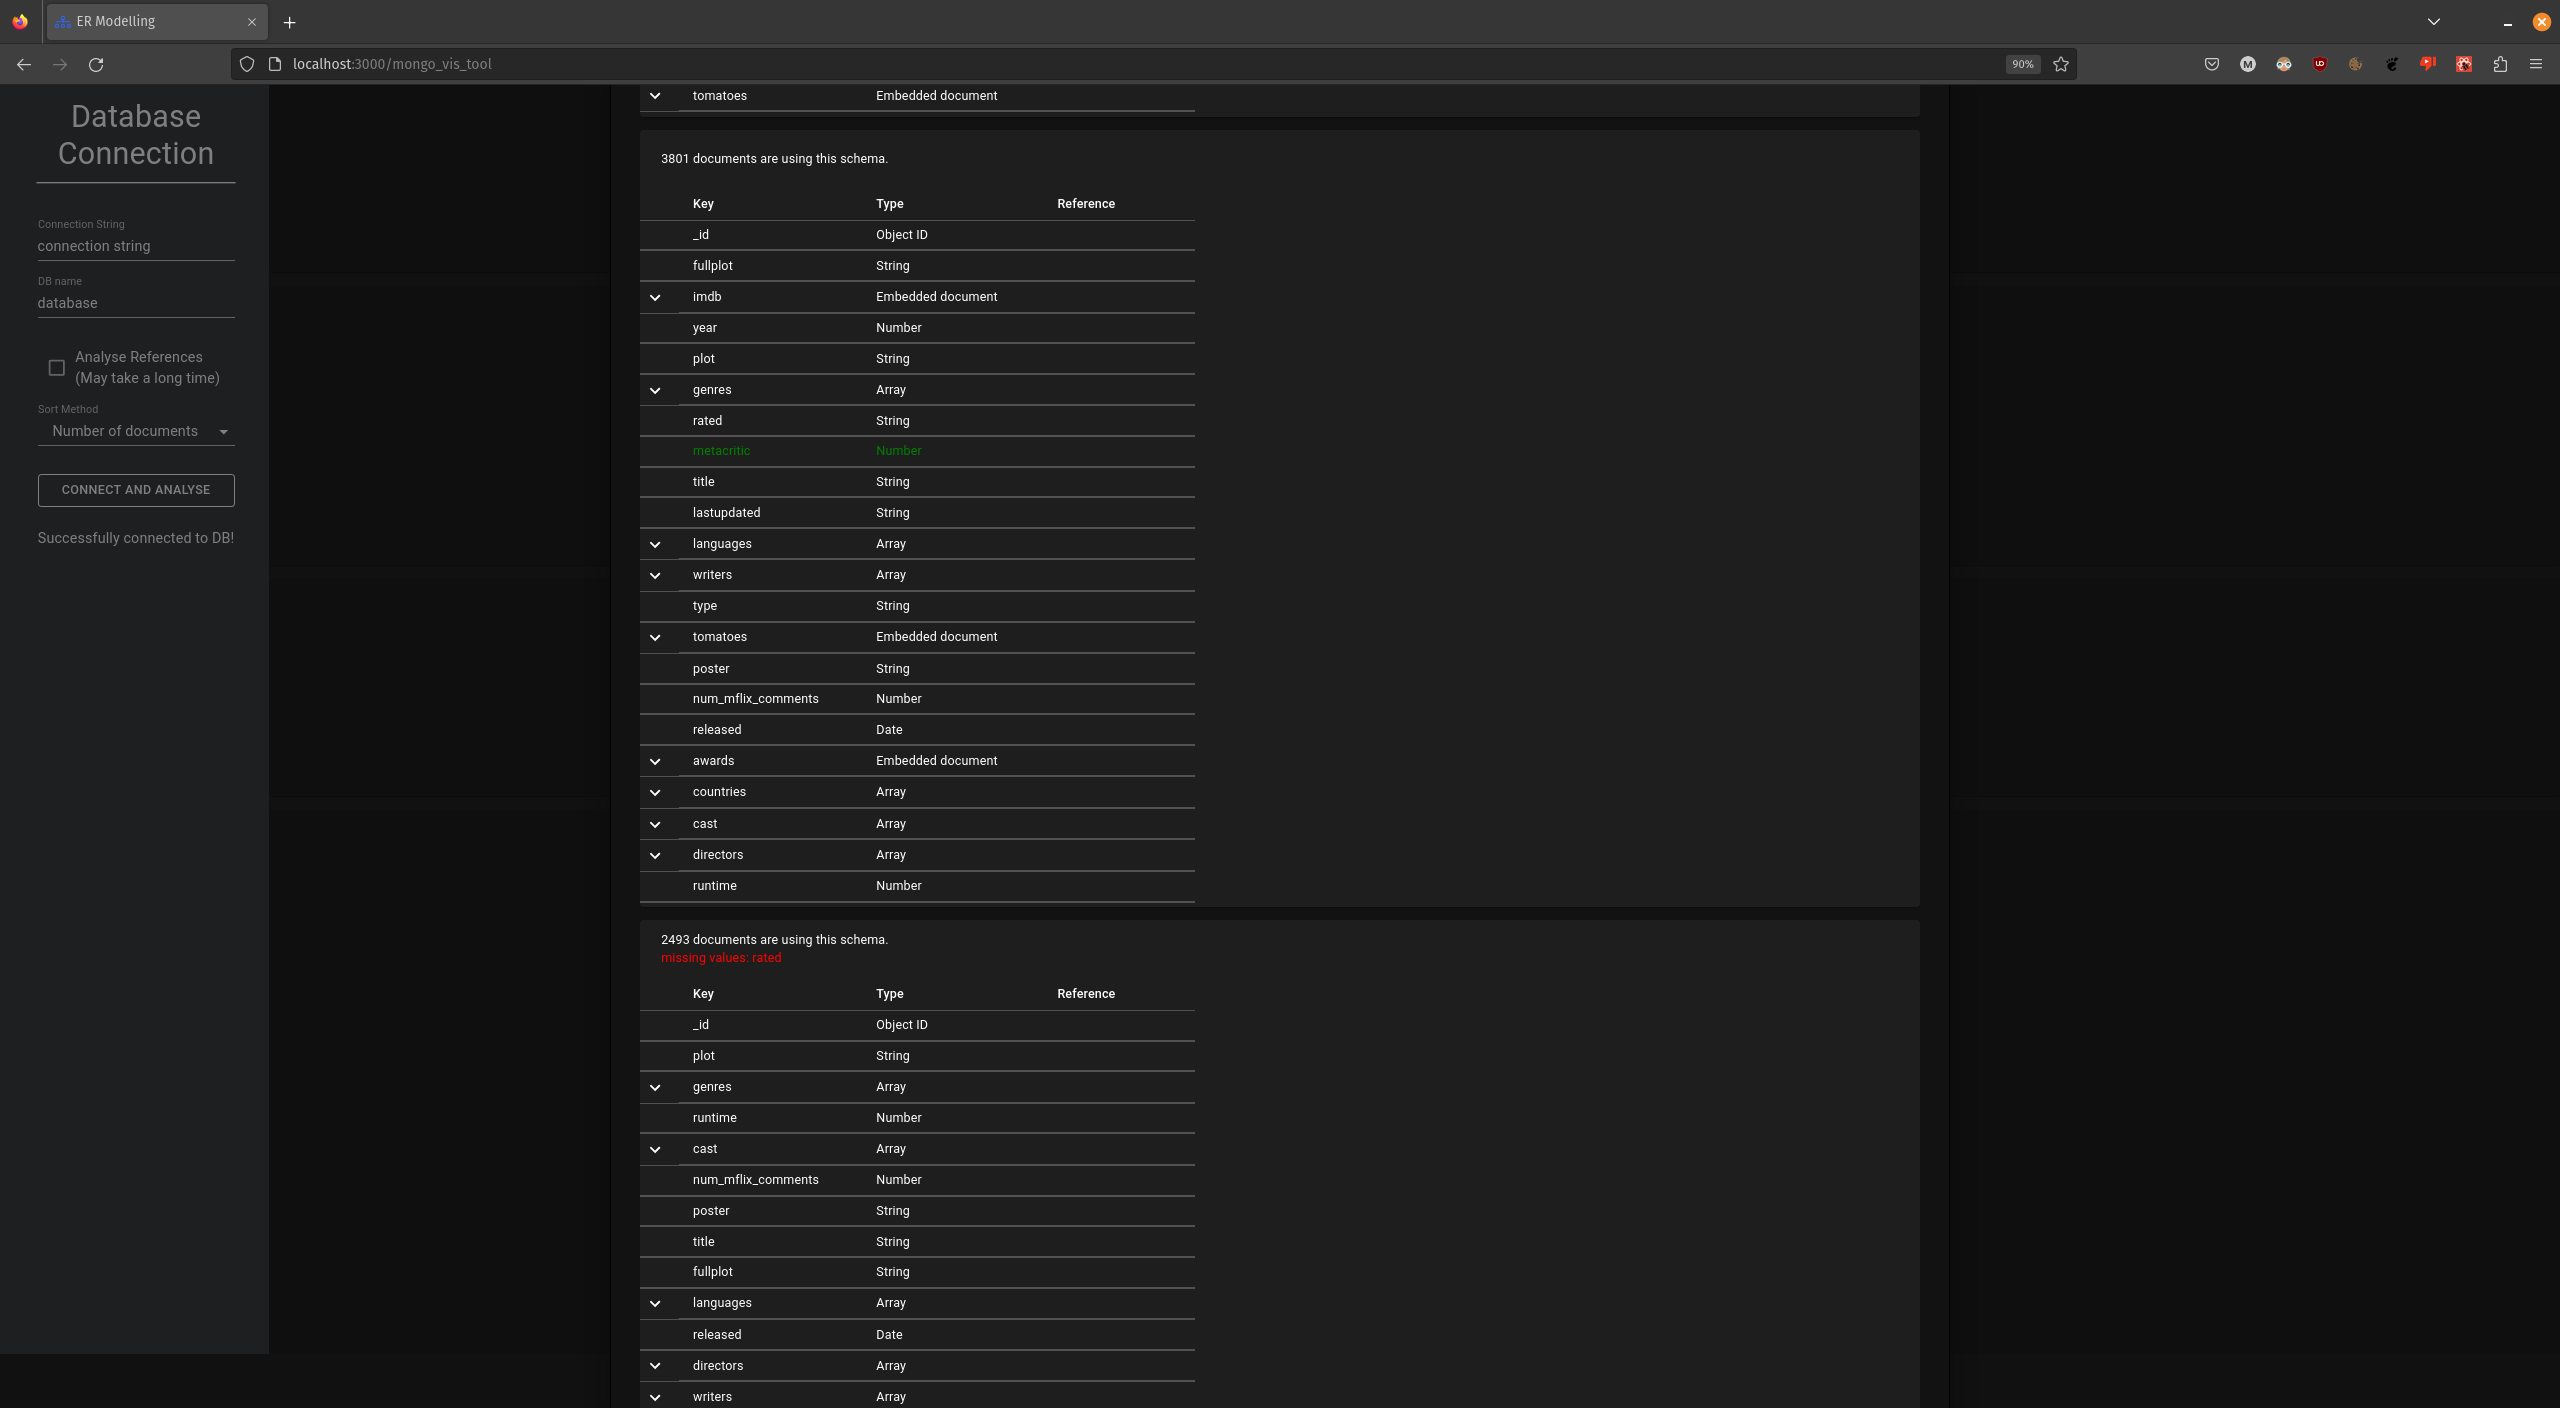
\includegraphics[width=\textwidth]{images/frontend_detail_view}
    \caption{Frontend DetailView Popup}
    \label{fig:frontend_detail_view}
\end{figure}

\subsection{Redux Store}
\label{sub:fe_redux}

Der Redux Store dient dem Speichern von States losgelöst von einzelnen React Komponenten.
Für das Speichern eines States wird ein sogenannter ContentSlice verwendet.
Die ContentSlices für das MongoDB Visualisierungstool sind alle grundsätzlich gleich aufgebaut:
Im initialState wird der Ausgangszustand des States definiert. 
Im Fall des MongoContentSlice wird initial collections auf null gesetzt.
Reducer sind Methoden, welche das Beschreiben des States erlauben.
in diesem Fall wurde der Reducer setCollections definiert, welcher es erlaubt, in collections das Argument documents zu schreiben.
Abschließend werden die actions und die reducer des ContentSlice exportiert, sodass diese global erreichbar sind.

\begin{lstlisting}[language=JavaScript, caption={MongoContentSlice},label={lst:fe_redux_slice}]
export const mongoContentSlice = createSlice({
    name: 'mongoContent',
    initialState: {
        collections: null
    },
    reducers: {
        setCollections: (state, documents) => {
            state.collections = documents
        }
    }
})

export const {setCollections} = mongoContentSlice.actions
export default mongoContentSlice.reducer
\end{lstlisting}

Auf diese Weise lassen sich schnell und einfach weitere ContentSlices definieren.
Um die ContentSlices zu verwenden, müssen diese nur noch in den Redux Store eingefügt werden.

\begin{lstlisting}[language=JavaScript, caption={Redux Store},label={lst:fe_redux_store}]
export const store = configureStore({
    reducer: {
        erContent: erContentSlice,
        relationalContent: relationalContentSlice,
        mongoContent: mongoContentSlice
    }
})

export default store;
\end{lstlisting}
